% !Mode:: "TeX:UTF-8" 



\BiSection{2.17}{Figures}

\fancyhead[R]{本题2.17由QC.Z完成}



解:

\scalebox{3}{(a)}

$I_D=\frac{1}{2}\mu_nC_{ox}\frac{W}{L}(V_{GS}-V_{TH})^2$




\begin{figure}[H] %H为当前位置,!htb为忽略美学标准,htbp为浮动图形
	\begin{minipage}{\linewidth}
		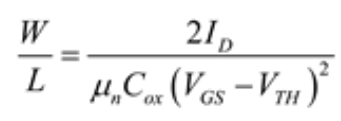
\includegraphics{2.17-1}
	\end{minipage}
\end{figure}


\begin{figure}[H] %H为当前位置,!htb为忽略美学标准,htbp为浮动图形
	\begin{minipage}{\linewidth}
		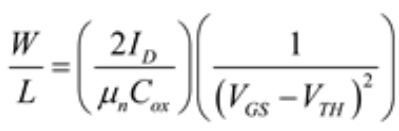
\includegraphics{2.17-2}
	\end{minipage}
\end{figure}







所以可画$y=a\times \frac{1}{x^2}$图像,令$a=1$

		\begin{figure}[H] %H为当前位置,!htb为忽略美学标准,htbp为浮动图形
	\begin{minipage}{\linewidth}
		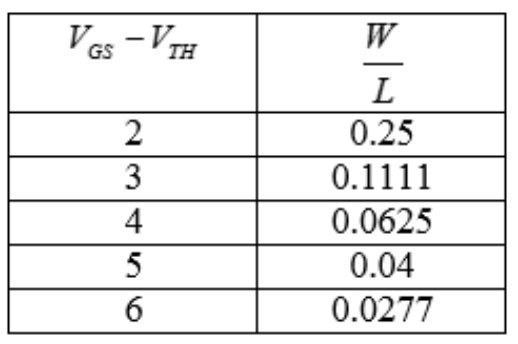
\includegraphics[width=1\linewidth]{2.17-3}
	\end{minipage}
	\caption*{表1} %最终文档中希望显示的图片标题
\end{figure}

		\begin{figure}[H] %H为当前位置,!htb为忽略美学标准,htbp为浮动图形
	\begin{minipage}{\linewidth}
		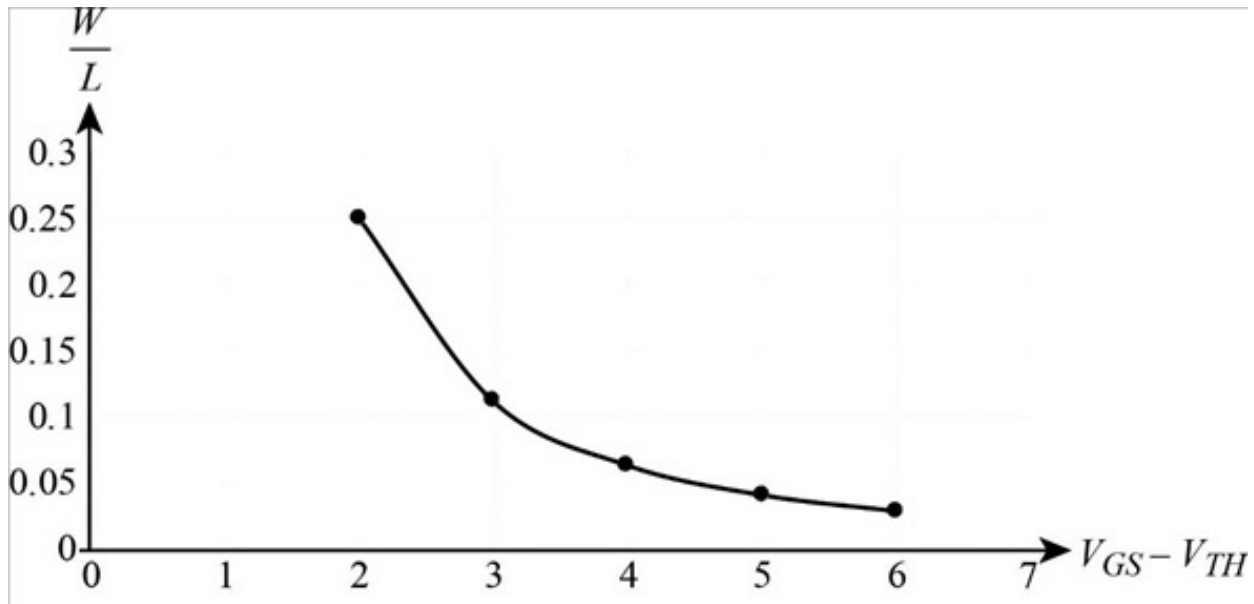
\includegraphics[width=1\linewidth]{2.17-4}
	\end{minipage}
	\caption*{图1} %最终文档中希望显示的图片标题
\end{figure}










\scalebox{3}{(b)}

$g_m=\mu_nC_{ox}\frac{W}{L}(V_{GS}-V_{TH})$


\begin{figure}[H] %H为当前位置,!htb为忽略美学标准,htbp为浮动图形
	\begin{minipage}{\linewidth}
		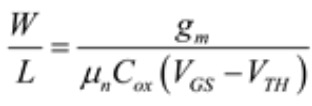
\includegraphics{2.17-5}
	\end{minipage}
\end{figure}


\begin{figure}[H] %H为当前位置,!htb为忽略美学标准,htbp为浮动图形
	\begin{minipage}{\linewidth}
		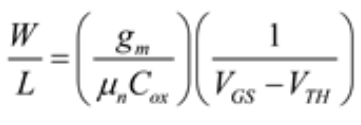
\includegraphics{2.17-6}
	\end{minipage}
\end{figure}



所以可画$y=a\times \frac{1}{x}$图像,令$a=1$


		\begin{figure}[H] %H为当前位置,!htb为忽略美学标准,htbp为浮动图形
	\begin{minipage}{\linewidth}
		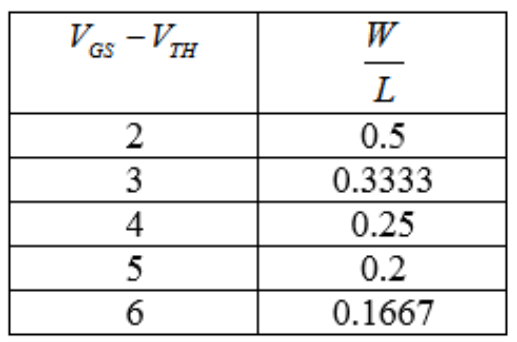
\includegraphics[width=1\linewidth]{2.17-7}
	\end{minipage}
	\caption*{表2} %最终文档中希望显示的图片标题
\end{figure}

\begin{figure}[H] %H为当前位置,!htb为忽略美学标准,htbp为浮动图形
	\begin{minipage}{\linewidth}
		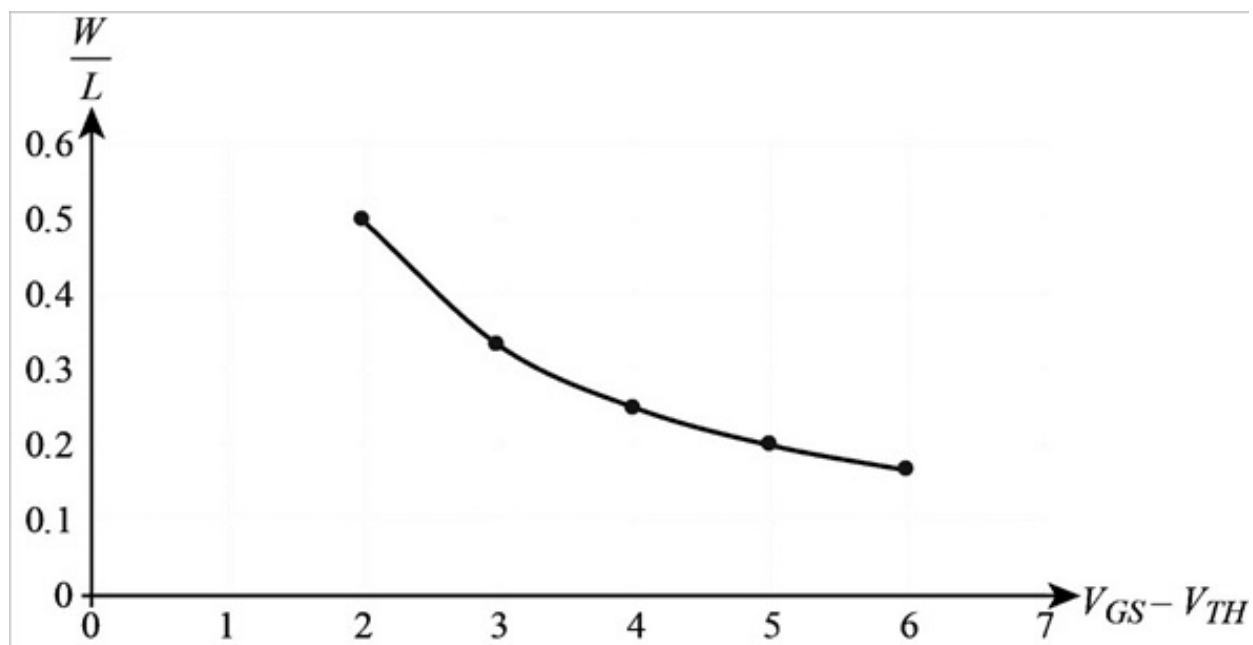
\includegraphics[width=1\linewidth]{2.17-8}
	\end{minipage}
	\caption*{图2} %最终文档中希望显示的图片标题
\end{figure}


